\documentclass[12pt]{article}

\usepackage{sbc-template}

\usepackage{graphicx,url}
\usepackage{float}
\usepackage{verbatim}
\usepackage[english]{babel}
\usepackage{xcolor}
\usepackage{hyperref}
\usepackage[T1]{fontenc}
\usepackage[utf8]{inputenc}

\sloppy

\title{Video Player Architecture for Virtual Reality on Mobile Devices}

\author{Adriano M. Gil, Afonso R. Costa Jr, Atacilio C. Cunha,\\ Thiago S. Figueira, Antonio A. Silva}

\address{SIDIA Instituto de Ci\^encia e Tecnologia
  (SIDIA)\\
  Manaus -- AM -- Brazil
\email{adriano.gil@sidia.com,afonso.costa@sidia.com,atacilio.cunha@sidia.com}
\email{thiago.figueira@sidia.com,antonio.arquelau@sidia.com}
}

\begin{document}

\maketitle

\section{Introduction}

 Virtual Reality (VR) applications provide great interaction with multimedia content. This kind of content becomes an unique experience for the end-user as applications work as a media gallery inside the VR environment such as the Samsung VR \cite{SVR}.

Those applications, which are usually built using 3D engines or frameworks, target mostly mobile devices like smartphones. In this scenario, it is important to define and follow a software architecture to organize the communication between the render and platform layers, thus provide better performance results.

This work proposes a high-performance architecture that can be implemented for video players on mobile platforms to run videos on VR environments. This architecture is evaluated using two 3D engines: (Unity \cite{Unity} and Samsung XR \cite{SXR}) in the Android platform. The methodology and initial experiments are in the following sections.

%This work proposes a high performance architecture which can be implemented for video players on mobile platforms to run videos on VR environments. This architecture is evaluated using two 3D engines (Unity\cite{Unity} and Samsung XR\cite{SXR}) on the Android platform. The methodology and initial experiments are described in the next sections. %

\section{Related Work}

Media consumption is a relevant activity for users in the digital world, content consumption has been growing according to \cite{repo2004users}. In \cite{hu2018kalgan} and \cite{smolic2009overview}, we find some examples of research made about video players. According to \cite{wild2018inaccessibility}, it is mandatory that a video player supports subtitle, audio description, media transcription, volume changing and color contrast.

%Consuming media is an activity of big relevance for users inside the digital world, where exists a growth number of content being consumed according to \cite{repo2004users}. In \cite{hu2018kalgan} and \cite{smolic2009overview}, are some examples of researches done about video player. According to \cite{wild2018inaccessibility} is mandatory that the video player supports subtitle, audio description, media transcription, volume changing and color contrast.%

\section{Methodology}

The methodology that is being followed to evaluate the proposed architecture is below:

%In a VR environment, will be made media types manipulation, for example: audio, image and video. With this options, the video media format was chosen for the experiments of this paper. So an architecture that has a good performance at mobile devices will be proposed. 

\begin{enumerate}
    \item Definition of the video format.
    \item Definition of ways to visualize the video in a virtual environment.
    \item Comparison between two different render implementations (Unity and SXR) in the Android platform (using two different devices).
    \item Comparison between two different native video players (ExoPlayer \cite{Exo} and Android Player \cite{AndroidVideoPlayer}).
\end{enumerate}

The chosen videos are 360-degree videos in the \textit{.mp4} format since this format is widely used in Android devices. The performance evaluation tool is the OVR Metrics Tool \cite{ovrmetrictool}, and the metric is frame-rate (FPS), which is most significant for the user experience.

\section{Architecture}

Seeking for an optimized way to use a video player in mobile virtual reality platforms, the architecture was divided into two main layers:

\begin{enumerate}
    \item Platform layer: native implementation to handle I/O operations and file system.
    \item Rendering layer: use of some render framework to turn visible inside the 3D virtual universe.
\end{enumerate}

This architecture (Figure \ref{fig-video-player-arch}) aims to (1) organize the communication between all modules present in the layers, (2) organize the code to be used by different render engines or different native players, and (3) provide good performance in all media codecs and texture renders. 

%The Platform layer is responsible for media consuming, file system, allocation and memory management. Some multimedia application that executes videos needs not only render digital media but allow user interact with this player. 

\begin{figure*}[h!]
    \centerline{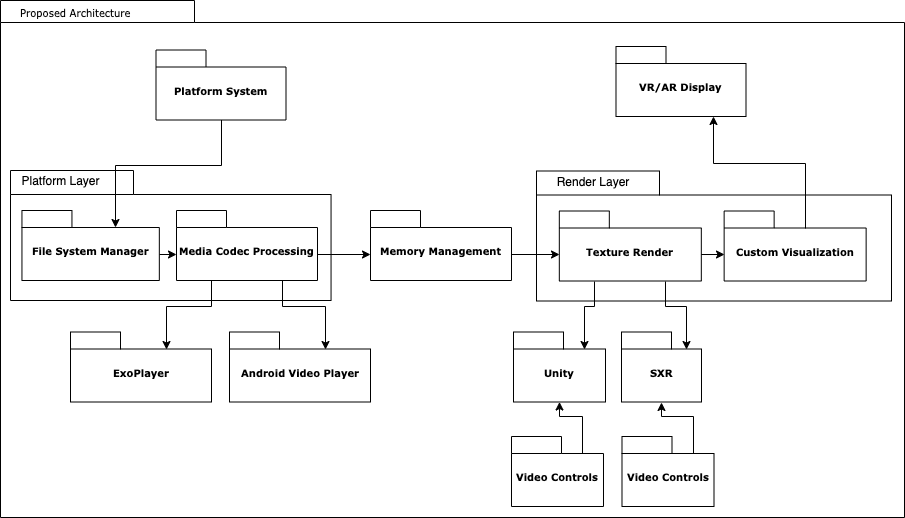
\includegraphics[scale=0.5]{images/ProposedArch.png}}
    \caption{Proposed architecture for Video Player}
    \label{fig-video-player-arch}
\end{figure*}

\subsection{Experiments and Results}

According to Figure \ref{SXR-graph} and Figure \ref{gallery-graph}, the SXR framework keeps 60 FPS in all test cases. However, the initial experiments have shown that the video player of VR Gallery (application developed in Unity) does not perform well. While in Samsung Galaxy S8, Gallery has variation between 55 and 60 FPS, in Samsung Galaxy S6 it stays between 40 and 50 FPS.

The graphs below shows the FPS performance of SXR.

\begin{figure*}[!h]
    \centerline{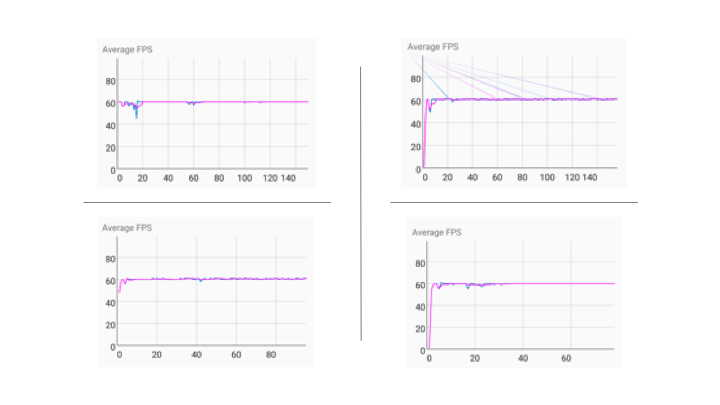
\includegraphics[scale=0.45]{images/SXR.png}}
    \caption{FPS on SXR}
    \label{SXR-graph}
\end{figure*}

This difference on both applications exists for the following reasons: SXR is an app that only has the video player while Gallery has many more features as well as background processes like providers and memory allocation lists; another significant difference is the virtual environment that is heavier in Gallery.

Even with the mentioned remarks, the user experience was not affected in any of the tests as the video player performed well. The user cannot perceive the difference between both applications and the frame-rate difference is unnoticeable in all tests.

The graphs below shows the FPS performance of Unity Framework.

\begin{figure*}[h!]
    \centerline{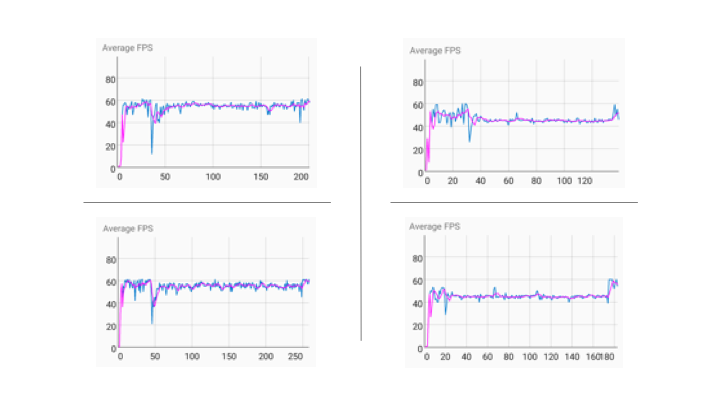
\includegraphics[scale=0.45]{images/Gallery.png}}
    \caption{FPS on VR Gallery}
    \label{gallery-graph}
\end{figure*}

\subsection{Conclusion / Next Steps}

According to the tests, the VR Gallery video player does not have good performance when compared to SXR, however the difference between the two can be explained by the fact that the VR Gallery is a complete and robust application, i.e. it has providers and animations. Even so, the video player of Gallery gives users a complete experience of a good performance video player in a VR environment.

For the full paper, other tests will be made using this architecture in Unity, but isolating the video player from any application. The same metrics will be used but the comparisons will be more directed to the architecture. Besides that, different native video players will be tested using the architecture as well.
\bibliographystyle{sbc}
\bibliography{hci-abstract}

\end{document}